\documentclass[a4paper,11pt]{article}
\usepackage[margin=1in]{geometry}
\usepackage{lastpage,fancyhdr,graphicx}
\graphicspath{ {/figure/} }
\usepackage{authblk}

\begin{document}
%\title{Mining sequential mobility patterns from semantic Twitter user trajectories}
\title{Sequential mobility patterns in people's daily life}
\author[1]{Junjun Yin}
\author[2]{Chao Zhang}
\author[1]{Shaowen Wang\thanks{shaowen@illinois.edu}}
\affil[1]{CyberGIS Center for Advanced Digtial and Spatial Studies}
\affil[2]{Department of Computer Science}
\affil[ ]{University of Illinois at Urbana-Champaign, IL, 61801, USA}

\renewcommand\Authands{ and }


\maketitle

\section*{\centering Abstract}
Understanding human mobility patterns 


\section*{Introduction}
Understanding detailed human mobility patterns in the urban settings is critical for a wide range applications, such as urban planning, traffic management, and even the spatial spread of disease.

On the other hand, to get 
However, the geo-located Twitter Data contains a variety of uncertainties, such spatial sparseness
To address these issue, this study implements a novel approach for getting the semantic trajectories by integrating detailed land use maps with geo-located Twitter data.

Emerging as a new source for mobility data, today's pervasive Location Based Social Media (LBSM) platforms (e.g., Twitter and Foursquare) offer continuous spatial Big Data streams with massive amount of detailed and frequently updated user digital traces in the form of real-world trails and footprints~\cite{thatcher2014}.
One significant advantage of LBSM data streams is the large spatial coverage, for example, researchers have used geo-located Twitter data for studying global mobility patterns~\cite{hawelka2014geo}, which is otherwise impossible by using other mobility datasets (e.g., GPS traces and mobile phone call records). 
In addition, the publicly available LBSM data streams offer unique opportunities for conducting reproducible scientific findings regarding the concerns of infringement on individual privacy, such as using mobile phone call records~\cite{giannotti2008mobility,crampton2014collect,Jurdak2015}.


\section*{Related Work}

\section*{Methods and Materials}

\subsection*{Geo-located Twitter Data}
In this study, the geo-located tweets were downloaded using the Twitter Streaming API, where we specified a geographical bounding box as an area-of-interest to retrieve all the geo-located tweets that fall within it.
To ensure the complete coverage over Great Britain, we have set the bounding box to British Isles (lower left coordinates in (latitude, longitude): (49.497, -14.854) and upper right coordinates: (61.186, 2.637)), which also includes the whole area of Ireland and a part of France.
We have implemented a data crawler and continuously collected 7-month data (1st June – 31st December, 2014) with over 101.8 million tweets and 60 GB in size.
During the data collection phase, the data crawler did not encounter any issue regarding whether it exceeds the data quota by the 1$\%$ policy mentioned in (Hawelka et al., 2014).
It means we have managed to download all the geo-located tweets for the given bounding box.
In particular, to showcase the overall spatial coverage of the collected geo-located tweets, a density map of the Twitter user locations in British Isles for July 2014 is shown in Figure 4, where the collected points alone visually reveal the geography of cities and countries, e.g. the clusters with high density of tweets (in color red) correspond to the skeleton of major cities.
  
\subsection*{The shape of human mobility}


\begin{figure}[ht]
	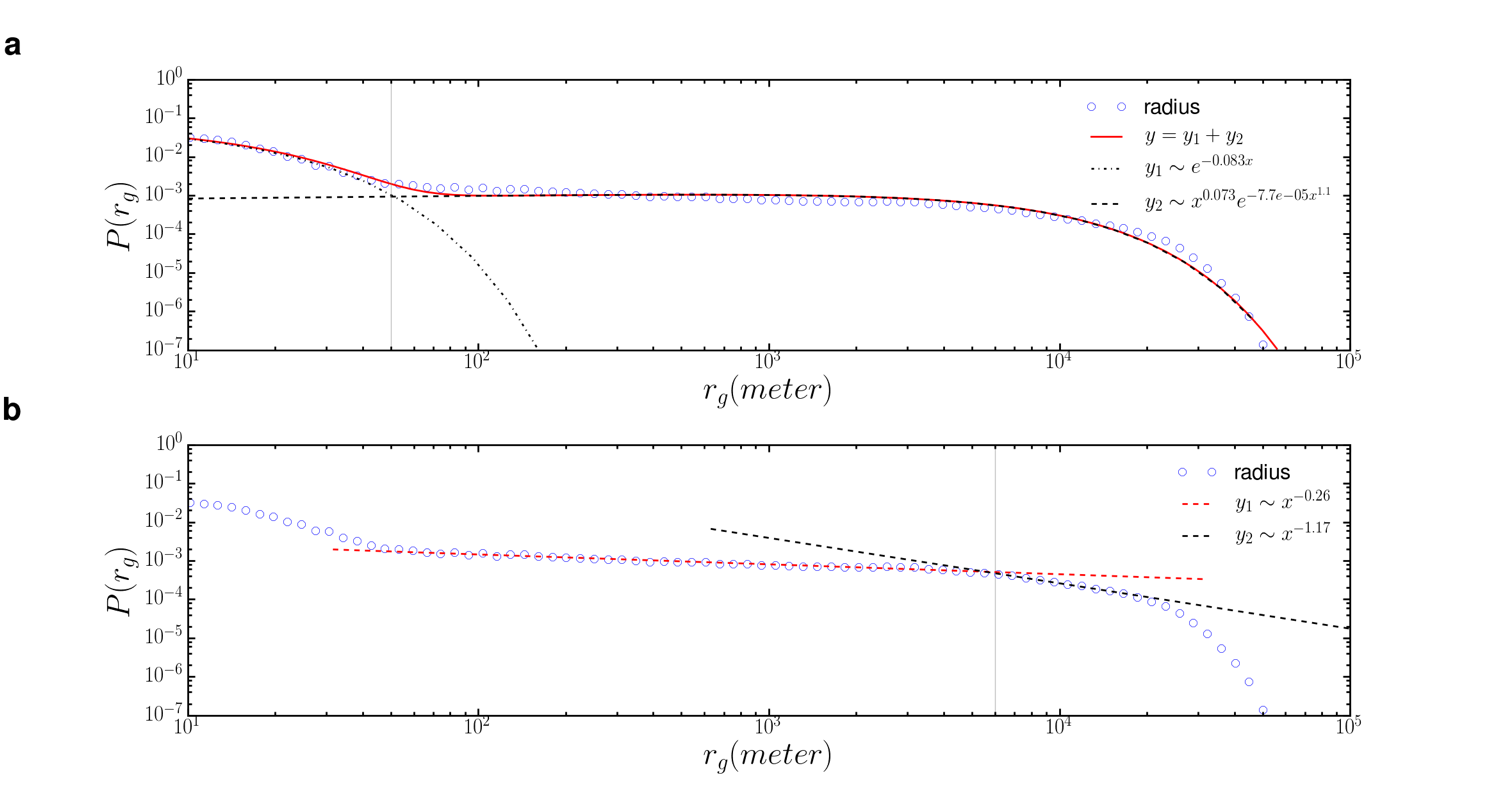
\includegraphics[width=1.0\linewidth]{./figure/gyration_chicago}
	\caption{{\bf The distribution of the radius of gyrations for Twitter users in Chicago}}
	\label{Fig_gyration}
\end{figure}


\begin{figure}[ht]
	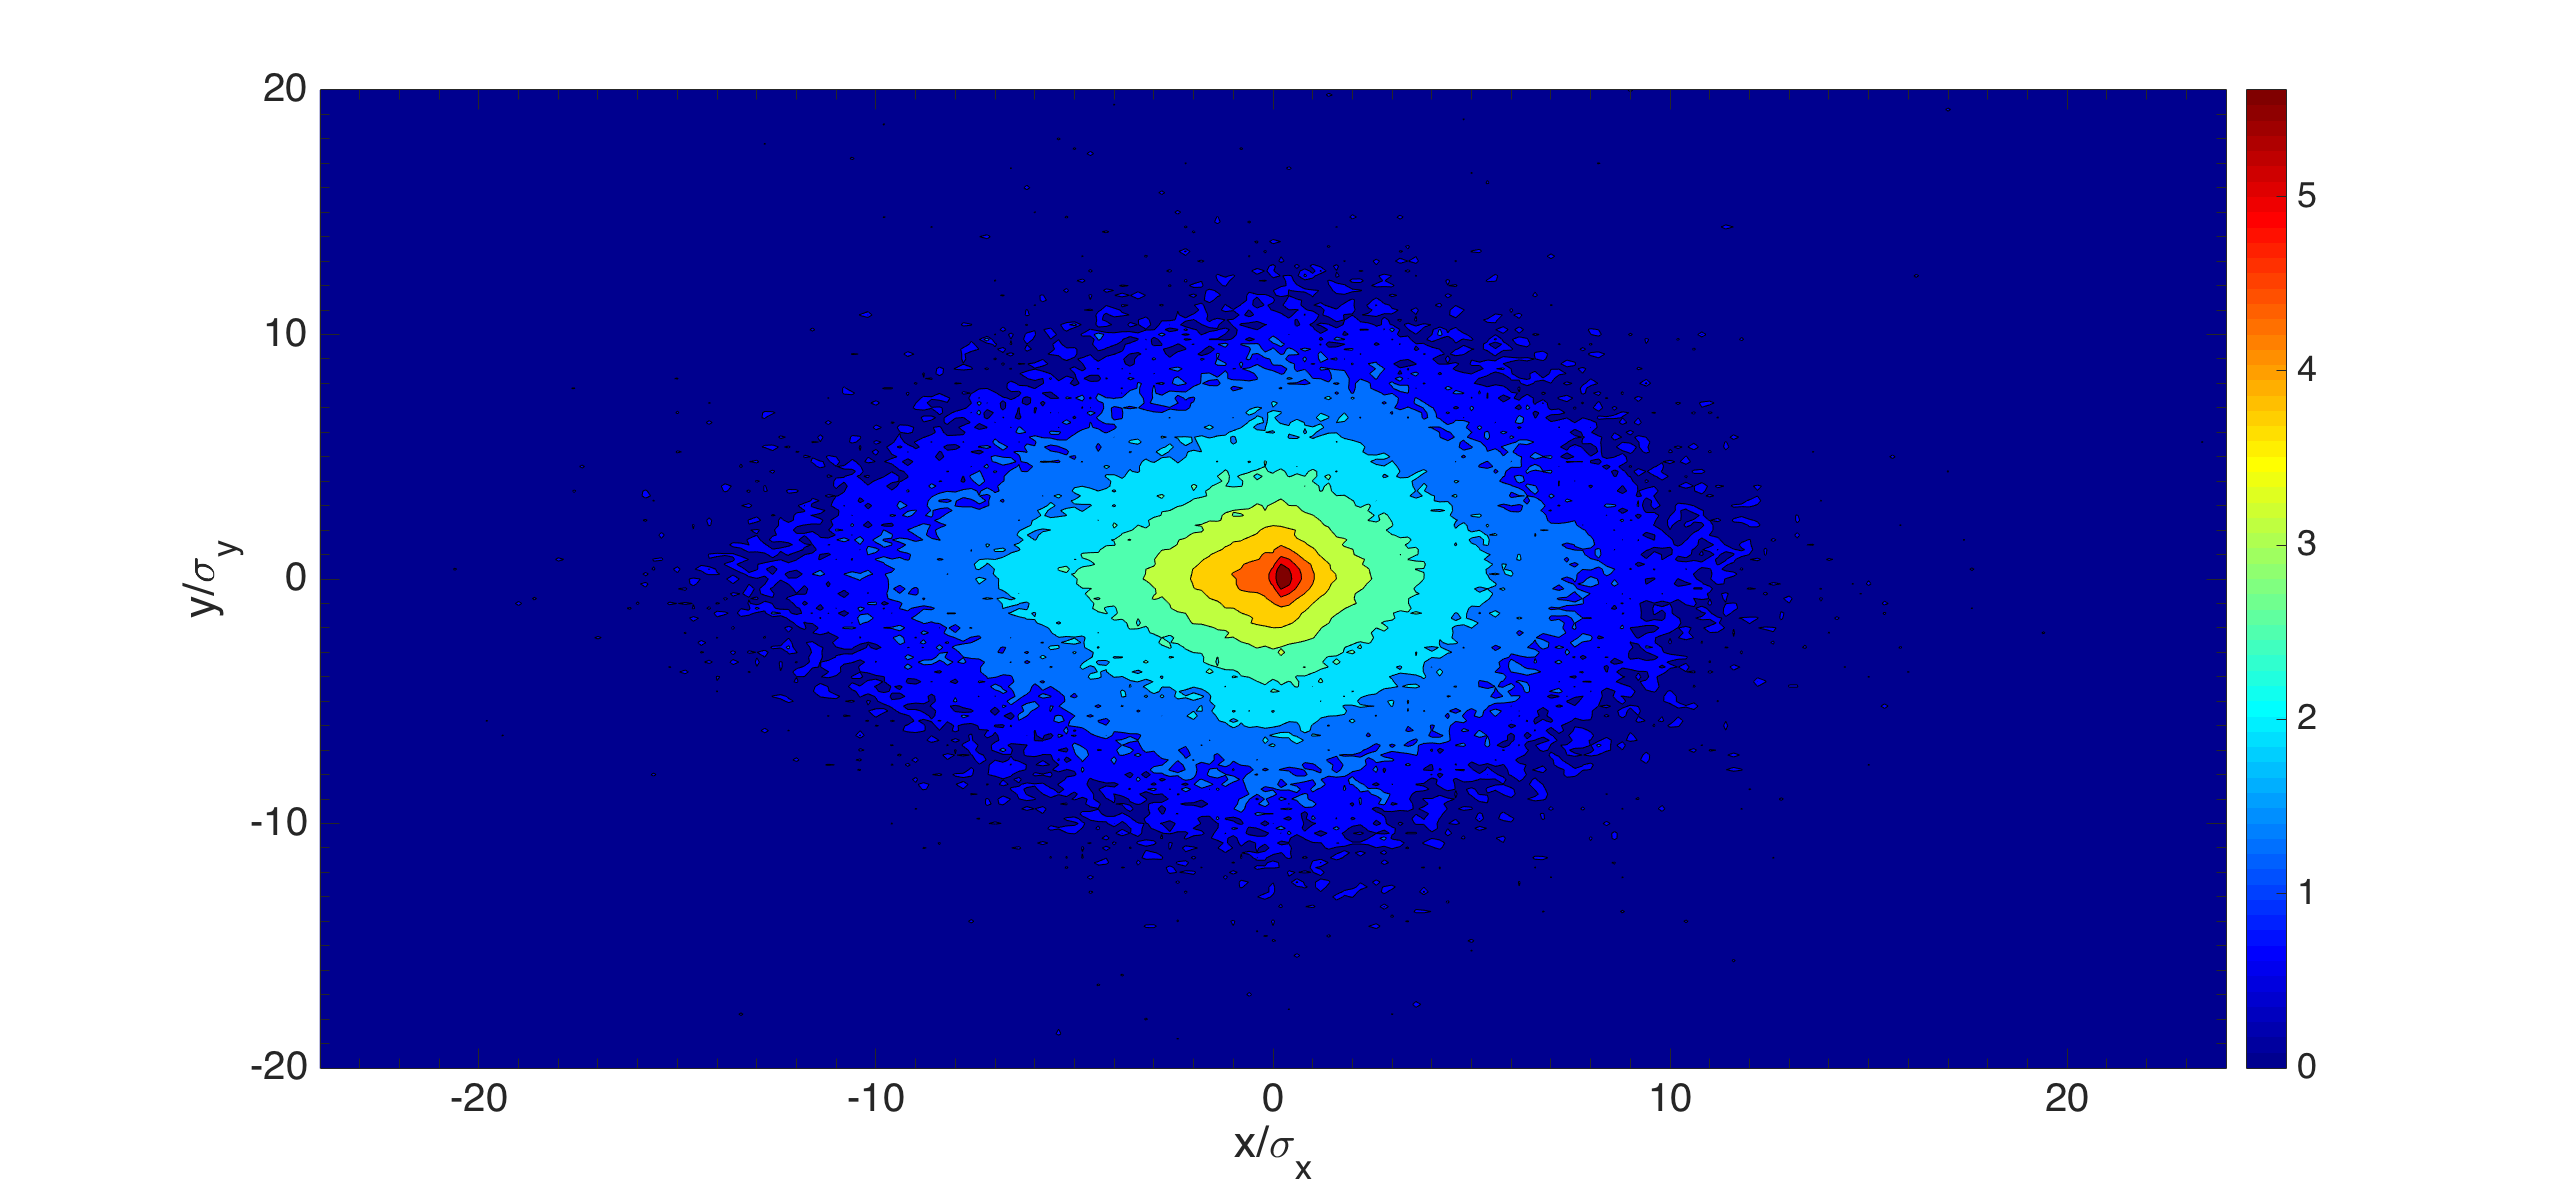
\includegraphics[width=1.0\linewidth]{./figure/Chicago_Shape}
	\caption{{\bf The shape of Twitter user mobility in Chicago for year 2014}}
	\label{Fig_shape}
\end{figure}

\begin{figure}[ht]
	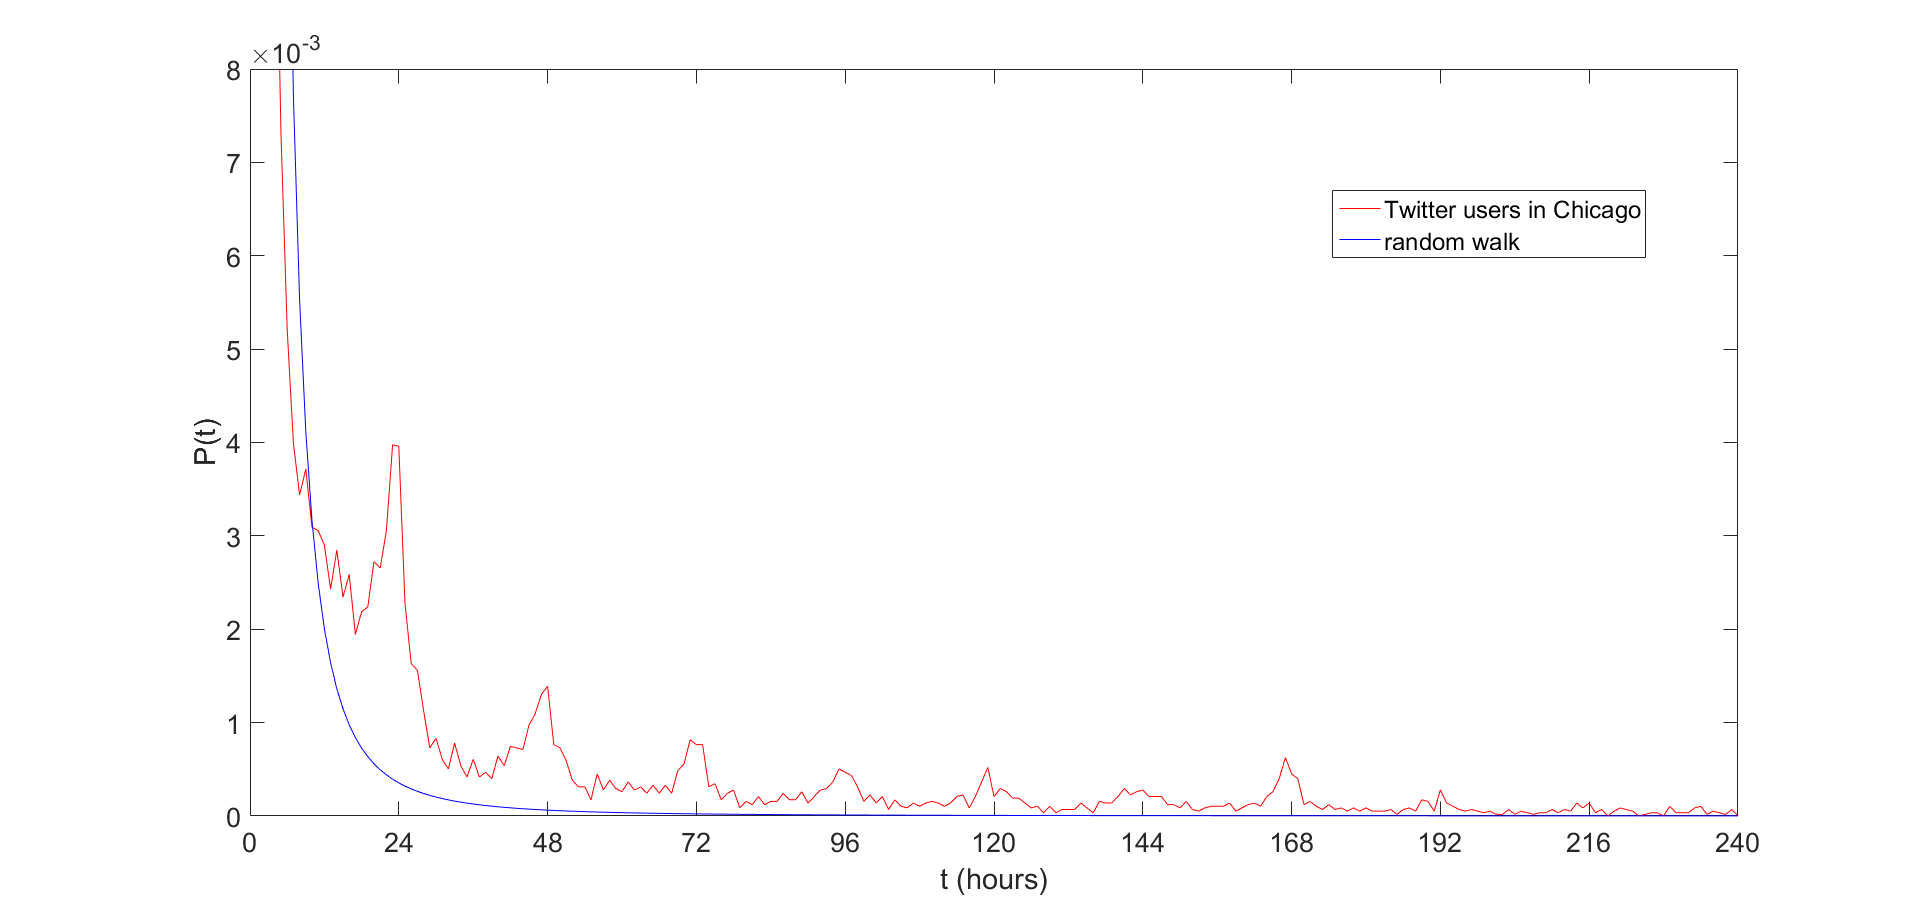
\includegraphics[width=1.0\linewidth]{./figure/firsttime}
	\caption{{\bf The shape of Twitter user mobility in Chicago for year 2014}}
	\label{Fig_shape}
\end{figure}




\section*{Results}

\section*{Discussion and Conclusion}


\end{document}